Заменив время на медленное $\tau = \varepsilon t$ в уравнениях (\ref{fullt}), получим (штрихом обозначается производная по $\tau$):
\begin{equation}
    \left\{
    \begin{aligned}
        \varepsilon \Lambda' &= U \sin \lambda - V \cos \lambda,
        &\quad
        \varepsilon \lambda' &= \alpha \Lambda,\\
        x' &= - \big( 2Fy+\frac{\partial U}{\partial y} \cos \lambda + \frac{\partial V}{\partial y} \sin \lambda \big),
        &\quad
        y' &= 2Fx+e_JG +\frac{\partial U}{\partial x} \cos \lambda + \frac{\partial V}{\partial x} \sin \lambda.
    \end{aligned}
    \right.
    \label{fulltau}
\end{equation}

Устремив $\varepsilon$ к нулю, получаем "медленную"\, систему:
\begin{equation}
    \left\{
    \begin{aligned}
        0 &= U \sin \lambda - V \cos \lambda,
        &\quad
        0 &= \alpha \Lambda, \\
        x' &= -\big( 2Fy+\frac{\partial U}{\partial y} \cos \lambda + \frac{\partial V}{\partial y} \sin \lambda \big),
        &\quad
        y' &= 2Fx+e_JG +\frac{\partial U}{\partial x} \cos \lambda + \frac{\partial V}{\partial x} \sin \lambda.
    \end{aligned}
    \right.
    \label{slowreal}
\end{equation}

Подставляя в (\ref{slowreal}) введенную ранее параметризацию листов медленного многообразия, получаем:
\begin{equation}
    \left\{
    \begin{aligned}
        x' &= - \big( 2Fy \pm \frac{\partial \beta}{\partial y} \big),
        &\quad
        y' &= 2Fx+e_JG \pm \frac{\partial \beta}{\partial x}.
    \end{aligned}
    \right.
    \label{slow_sys}
\end{equation}
Знаки "$+$" и "$-$" соответсвуют $M_{0,+}$ и $M_{0,-}$ соответственно.

Данная система является гамильтоновой с гамильтонианом:
$$H_S = F(x^2+y^2) + e_JGx \pm \beta(x,y),$$
и имеет одну степень свободы, что приводит к ее интегрируемости.

На каждом из листов медленного многообразия такая система единственное положение равновесия:
$$
y_0^{\pm} = 0,\quad
x_0^{\pm} = \frac{e_J (\pm D - G)}{2(F \mp C)}.
$$

Линеаризуя правую часть уравнений в окрестности этой точки, получаем что собственные значения матрицы линеаризации имеют вид:
$$\zeta = \pm \sqrt{- \left( 2F \pm 2C \pm \frac{2Cx_0^{\pm}+e_JD}{|U(x_0^{\pm},0)|} \right)\big( 2F \mp 2C \big)} \in \mathbb{R},$$
причем, учитывая значения констант, они являются чисто вещественными, что позволяет сказать о неустойчивости данного положения равновесия на обоих листах.

Как и в случае маятника, эти неустойчивые положения равновесия обладают двумерными сепаратрисами, заполненными сепаратрисными решениями, асимптотически приближающимися к положениям равновесия при $\tau\to \pm\infty$. Для их нахождения рассмотрим линию критического уровня гамильтониана $H_S(x,y) = H_S(x_0^{\pm},y_0^{\pm})$, соответствующего неподвижной точке:
$$H_S(x_0^{\pm},y_0^{\pm}) = F(x^2+y^2)+e_JGx \pm \beta(x,y).$$

\begin{figure}[H]
\centering
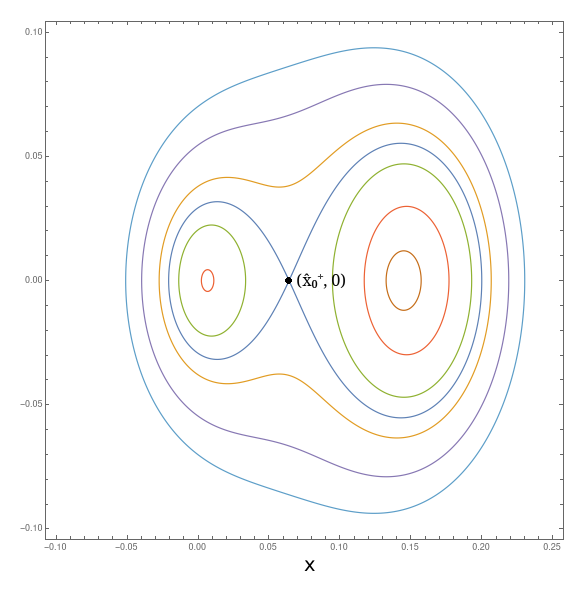
\includegraphics[scale=0.4]{../img/Hlines.png}
\caption{Линии уровня гамильтониана $H_S$ на $M_{0,+}$. На $M_{0,-}$ линии уровня имеют аналогичный вид}
\label{levels_slow}
\end{figure}

Сделав замену $x = x_0^{\pm} + h$ и упростив выражение, получаем:
\begin{multline}
(F^2-C^2)(h^2+y^2)^2+2(h^2+y^2) \big(U(x_0^{\pm}, y_0)+h(2Cx_0^{\pm}+e_JD) \big) (\pm F - C)+\\ 
+ y^2 \big(4U(x_0^{\pm},y_0^{\pm})C-(2Cx_0^{\pm}+e_JD)^2 \big) = 0.
\label{eight}
\end{multline}
Сделаем инверсию относительно единичной окружности: $X=\frac{h}{h^2+y^2}$, $Y=\frac{y}{h^2+y^2}$. Тогда уравнение (\ref{eight}) принимает вид:
$$(F^2-C^2)+AX^2+2BX+(A+\delta)Y^2=0,$$
где
$$A = 2 U(x_0^{\pm}, y_0^{\pm})(\pm F - C),$$
$$B = (2Cx_0^{\pm}+e_J D)(\pm F - C),$$
$$\delta = -(2Cx_0^{\pm}+e_J D)^2.$$
Если ввести новые переменные:
$$\xi  = \left( X+\frac{B}{A} \right) \sqrt{\frac{A}{F^2-C^2-\frac{B^2}{A}}} \equiv \omega \left( X+\frac{B}{A} \right),$$
$$\eta = Y \sqrt{\frac{-(A+\delta)}{F^2-C^2-\frac{B^2}{A}}} \equiv \sigma Y,$$
то уравнение критического уровня может быть переписано следующим образом:
\begin{equation}
\label{hyper}
\xi^2-\eta^2=1.
\end{equation}
Таким образом, в переменных $(\xi, \eta)$ линия уровня гамильтониана $H_S(x,y) = H_S(x_0^{\pm},y_0^{\pm})$ есть гипербола. В первоначальных переменных  $(x, y)$, т.е. до инверсии относительно единичной окружности, данная кривая имеет форму "восьмерки"\, (см. рис. \ref{levels_slow}).

Введем следующую параметризацию полученной кривой с помощью переменной $f$:
$$\xi = \ch f,$$
$$\eta = \sh f,$$
$$\xi^2-\eta^2 = \ch^2f - \sh^2f = 1.$$
Теперь для нахождения сепаратрисного решения необходимо определить зависимость $f$ от времени $\tau$. Для этого рассмотрим:
\begin{equation}
\label{der_x_1}
x' = \frac{\partial x}{\partial X}X'+\frac{\partial x}{\partial Y}Y' = \frac{Y^2-X^2}{(X^2+Y^2)^2}X' + \frac{-2XY}{(X^2+Y^2)^2}Y' = f' \sh f \frac{Q(\ch f)}{P^2(\ch f)},
\end{equation}
где
$$P(\ch f) \equiv X^2+Y^2 = \ch^2 f \left( \frac{1}{\omega^2} + \frac{1}{\sigma^2} \right) + \frac{-2B }{\omega A}\ch f + \left( \frac{B^2}{A^2}-\frac{1}{\sigma^2} \right),$$

$$Q(\ch f) \equiv  -\frac{\ch^2 f}{\omega} \left( \frac{1}{\omega^2}+\frac{1}{\sigma^2} \right) + \frac{2B}{A} \ch f \left( \frac{1}{\sigma^2}+\frac{1}{\omega^2} \right) - \frac{1}{\omega} \left( \frac{1}{\sigma^2} + \frac{B^2}{A^2} \right).$$

С другой стороны, подставляя (\ref{eight}) в первое уравнение системы (\ref{slow_sys}), получаем:

$$x' = -\left( 2Fy \pm \frac{\partial \beta}{\partial y} \right) = -2Fy \mp \frac{1}{\beta} \left( U \frac{\partial U}{\partial y} + V \frac{\partial V}{\partial y} \right) = $$

$$ = \frac{y \Big(2(C^2-F^2)(x^2+y^2) + 2x(2Cx_0+e_J D)(C \mp F) + (2Cx_0+e_J D)^2 + 2U(x_0, y_0)(-C \mp F)  \Big)}{F(x^2+y^2) \pm U(x_0, y_0) \pm x(2Cx_0+e_J D)}.$$

Тогда в терминах переменной $f$ получаем
\begin{equation}
\label{der_x_2}
x' = \frac{\sh f}{\sigma P(\ch f)} \frac{R(\ch f)}{S(\ch f)},
\end{equation}
где
$$R(\ch f) \equiv P(\ch f) \left( 2 U(x_0,y_0)(-C \mp F)+(2Cx_0+e_J D)^2 \right) +$$ 
$$ + 2 \left( \frac{\ch f}{\omega} - \frac{B}{A} \right)(2Cx_0 + e_J D)(C \mp F) + 2(C^2-F^2),$$
$$S(\ch f) \equiv \pm U(x_0,y_0) P(\ch f) \pm \left( \frac{\ch f}{\omega} - \frac{B}{A}\right) (2Cx_0+e_J D) + F.$$
Сравнивая выражения (\ref{der_x_1}) и (\ref{der_x_2}), получаем дифференциальное уравнение на $f$:
\begin{equation}
\label{der_f}
f' = \frac{1}{\sigma} \frac{R(\ch f) P(\ch f)}{S(\ch f)Q(\ch f)}.
\end{equation}
Заметим, что $P, Q, R, S$ являются полиномами второго порядка переменной $\ch f$.
Интегрируя уравнение (\ref{der_f}), имеем:
\begin{equation*}
\tau -\tau_0 = \sigma \int_{f_0}^f \frac{S(\ch f) Q(\ch f)}{R(\ch f)P(\ch f)} df = 
\end{equation*}
\begin{equation} = (f-f_0)\frac{\mp 2U(x_0^{\pm}, y_0^{\pm}) \frac{\sigma}{\omega}}{2U(x_0^{\pm},y_0^{\pm})(-C \mp F)+(2Cx_0^{\pm} + e_J D)^2} + \sigma \int_{f_0}^f \frac{L(\ch f)}{R(\ch f) P(\ch f)} df,
\label{f_tau}
\end{equation}
где $L$ некоторый полином 3 степени.

\begin{utv}
На обоих листах $M_{0,k}, k=+,-$ медленная система (\ref{slow_sys}) имеет неустойчивое положение равновесия $(x,y) = (x_0^{\pm},y_0^{\pm})$. Это положение равновесия порождает двумерную сепаратрису, заполненную решениями вида:
$$x(\tau,\tau_{0}) = x_0 + \frac{\frac{\ch \big( f(\tau-\tau_{0}) \big)}{\omega} - \frac{B}{A}}{P \Big(\ch \big( f (\tau-\tau_{0}) \big) \Big)},$$
$$y(\tau, \tau_{0}) = \frac{\sh \big( f(\tau-\tau_{0}) \big)}{\sigma P\Big(\ch \big( f (\tau-\tau_{0}) \big) \Big)},$$
где $\tau_{0}\in \mathbb{R}$, а функция $f(\tau)$ задается выражением (\ref{f_tau}).
\end{utv}